% Preamble
\documentclass[11pt]{article}

% Packages
\usepackage{amsmath}
\usepackage{mathtools}
\usepackage{ragged2e}
\usepackage [utf8]{inputenc}
\usepackage{blindtext}
\usepackage{wrapfig}
\usepackage{xcolor}
\usepackage {polski}
\usepackage{multicol}
\usepackage[a4paper, total={5.7in, 8in}]{geometry}
\usepackage{graphicx}
\usepackage{amstex}
\usepackage{csvsimple}
\usepackage{changepage}
\usepackage{enumitem}
\usepackage[english]{babel}
\usepackage{biblatex}
\usepackage{caption}
\usepackage{indentfirst}
\usepackage{epstopdf-base}
\usepackage{textcomp}
\usepackage{wasysym}

% Document
\begin{document}
%    Nagłówek
    \begin{flushleft}
        Maciej Pierzchała 282 934 \hfill Data wykonania ćwiczenia:\\
        Filip Kubecki 272 655 \hfill 5 listopada 2024r\\
        Grupa: Wtorek 10:35 \\
    \end{flushleft}
    \begin{center}
        \Large\textbf{Laboratorium 5}\\
        \textbf{Charakteryzacja czujników wilgotności}
    \end{center}
    \hfill
%    Treść
    \section{Spis przyrządów}
    \par{
        Do wykonania ćwiczenia wykorzystano:
        \begin{itemize}
            \setlength\itemsep{0em}
            \item[-] Pojemnościowy czujnik wilgotności
            \item[-] Impedancyjny czujnik wilgotności
            \item[-] Multimetr cyfrowy Sigilent SDM 3055
            \item[-] Termohigrobarometr LAB-EL LB706B
            \item[-] Kolby kuliste z roztworami odpowiednich soli
        \end{itemize}
    }
    \section{Przebieg i cele doświadczenia}
    \par Ćwiczenie polegało na pomiarze wilgotności powietrza przy pomocy czujnika pojemnościowego, impedancyjnego oraz
    przy pomocy termohigrobarometru. Mierzono wilgotność pomietrza w pomieszczeniu oraz wewnątrz kolb zawierających roztwory
    odpowiednich soli które pozwalały na ustalenie stabilnej wilgotności na odpowiednich poziomach.\\
    \indent Celami ćwiczenia było zapoznanie się z budową oraz zasadą działania czujnika pojemnościowego oraz impedancyjnego,
    zapoznanie się z metodyką otrzymywania atmosfery pomiarowej o określonej wilgotności, wyznaczenie krzywej kalibracyjnej oraz określenie
    wilgotności atmosfery otoczenia.

    \section{Obliczenia i analiza wyników}
    \par Na podstawie pomiarów wyznaczono charakterystyki $C=f(RH)$ dla czujnika pojemnościowego oraz impedancyjnego.
    Na wykresach charakterystyk zamieszczono również równanie prostej kalibracyjnej oraz wartość współczynnika $R^2$.\\
    \noindent\makebox[\textwidth]{
        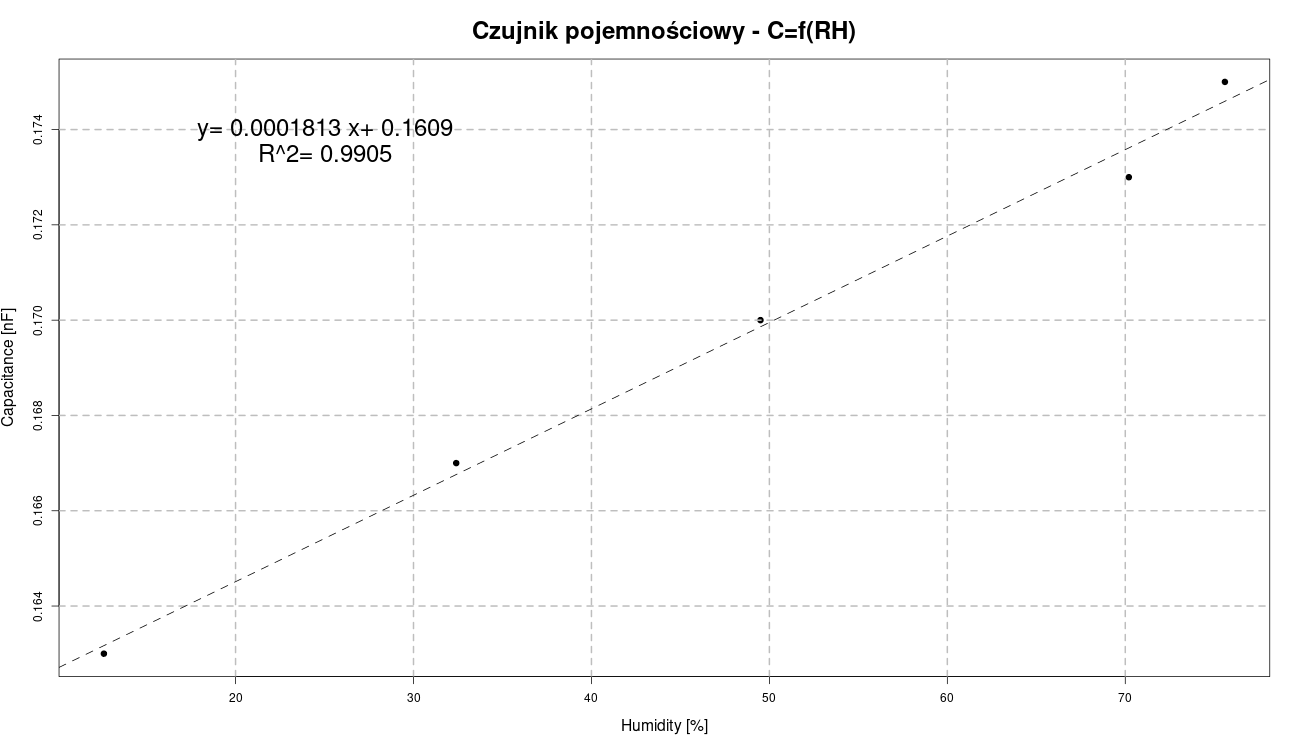
\includegraphics[scale = 0.35]{/home/bork/IdeaProjects/LatexProjects/src/PodstawyTechnikiSensorowej/Lab5/Img/capCRH.png}}
    \noindent\makebox[\textwidth]{
        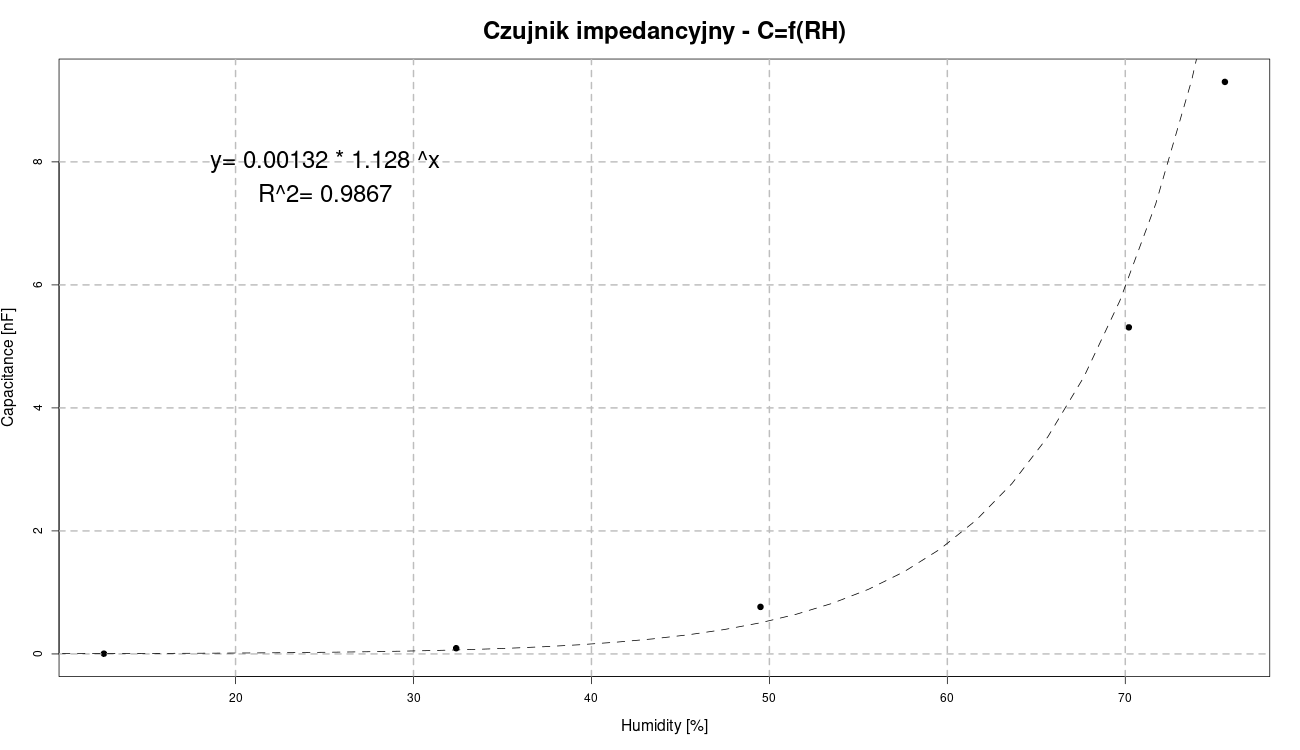
\includegraphics[scale = 0.35]{/home/bork/IdeaProjects/LatexProjects/src/PodstawyTechnikiSensorowej/Lab5/Img/impCRH.png}}
    \noindent\makebox[\textwidth]{
        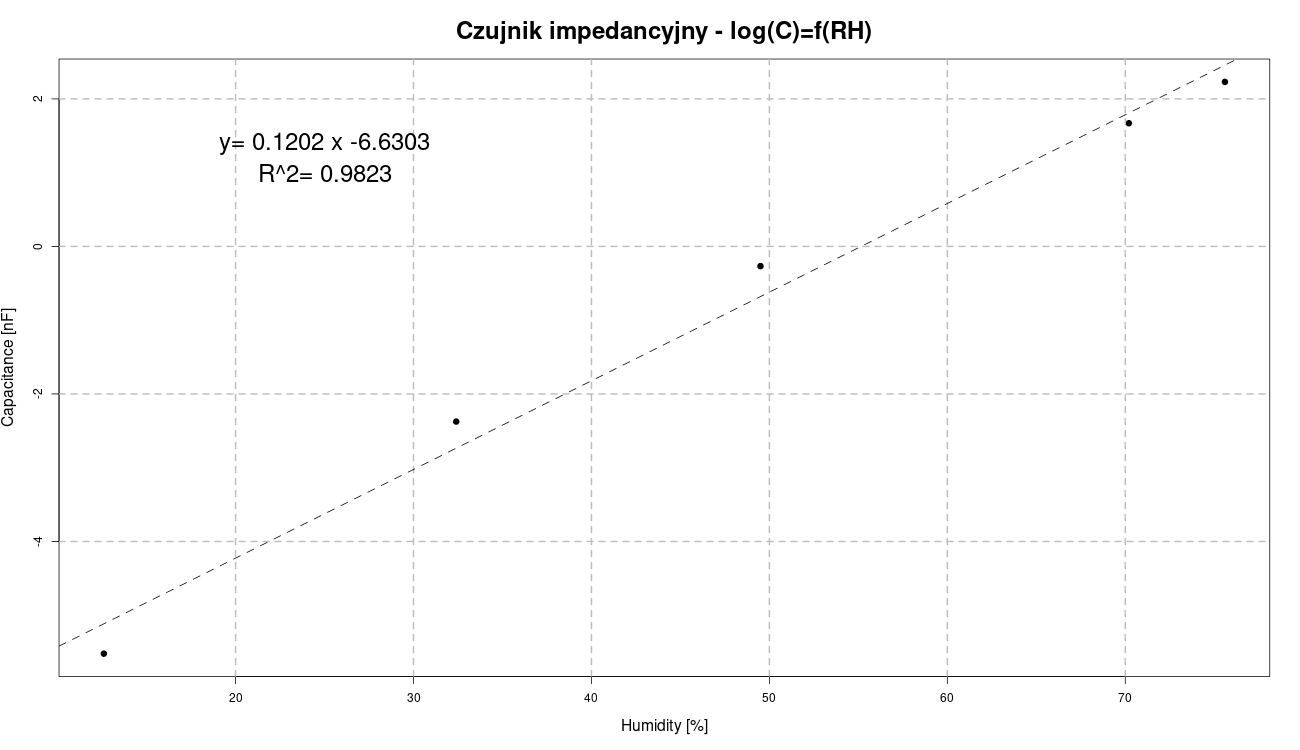
\includegraphics[scale = 0.35]{/home/bork/IdeaProjects/LatexProjects/src/PodstawyTechnikiSensorowej/Lab5/Img/impLogCRH.png}}

    \indent Przy pomocy zmierzonej temperatury pomieszczenia wyznaczono ciśnienie pary nasyconej dla warunków sali:
    \begin{gather}
        p_n=0.61121*\exp((18.678-\frac{T}{234.5})(\frac{T}{257.14+T}))
    \end{gather}
    Dla naszej temperatury pomieszczenia równej 24.8 [$C^\circ$]:
    \begin{gather}
        p_n=0.61121*\exp((18.678-\frac{24.8}{234.5})(\frac{24.8}{257.14+24.8}))=3.13095 [kPa]
    \end{gather}
    \noindent Wartość ta jest bliska wartości tablicowej więc można założyć poprawność obliczenia.\\
    \noindent Ciśnienie cząstkowe pary wodnej obliczamy przekształcając poniższy wzór:
    \begin{gather}
        RH=\frac{p_w}{p_n}\cdot 100\% \\
        p_w=\frac{RH\cdot p_n}{100\%}
    \end{gather}
    Przykładowo do atmosfery z solami LiCl (RH - współczynnik RH skorygowany dla temperatury otoczenia):
    \begin{gather}
        p_w=\frac{11.3\% \cdot 3.13095[kPa]}{100\%}=0.3537974[kPa]=353.7974[Pa]
    \end{gather}
    \indent Wilgotność atmosfery sali na podstawie wartości zmierzonych obliczamy przekształcając równanie prostej dla krzywych
    kalibracyjnych:
    \begin{gather}
        C=a*RH+b \\
        RH=\frac{C-b}{a}
    \end{gather}
    \noindent Dla czujnika pojemnościowego:
    \begin{gather}
        RH=\frac{0.171-0.1608843}{0.0001813}=55.79537[\%]
    \end{gather}
    \noindent Dla czujnika impedancyjnego wykorzystujemy wzór:
    \begin{gather}
        C=b*a^{RH} \\
        RH=\log_{a}{\frac{C}{b}}
    \end{gather}
    \noindent Dla pomiaru wilgotności otoczenia:
    \begin{gather}
        RH= \log_{1.128}{\frac{0.4}{0.0132}}=47.5334[\%]
    \end{gather}
    \indent Pomiary te odbiegają od wartości zmierzonej przez termohigrobarometr. Wartość dla czujnika pojemnościowego może różnić się
    z powodu zmian wilgotności powietrza w trakcie zajęć. Może to mieć znaczące znaczenie gdyż pomiar termohigrobarometrem wykonano na początku
    zajęć a pomiar czujnikiem pojemnościowym pod koniec kiedy otworzono już okna (zapomniano dokonać pomiaru wilgotności pomieszczenia na początku zajęć).
    W przypadku czujnika impedancyjnego wynik jest bardzo zbliżony do wartości podanej przez termohigrobarometr. Wartości te zostały zmierzone zaraz
    po sobie co pozwoliło osiągnąć ten efekt.\\
    \indent Wyznaczono czas odpowiedzi oraz czas powrotu dla czujnika indukcyjnego dla roztworu MgCl3 (najlepsza krzywa z wszystkich).
    Czas odpowiedzi oraz powrotu wyznaczono wykorzystując metody analityczne a wniki obliczeń przedstawiono na wykresach:
    \noindent\makebox[\textwidth]{
        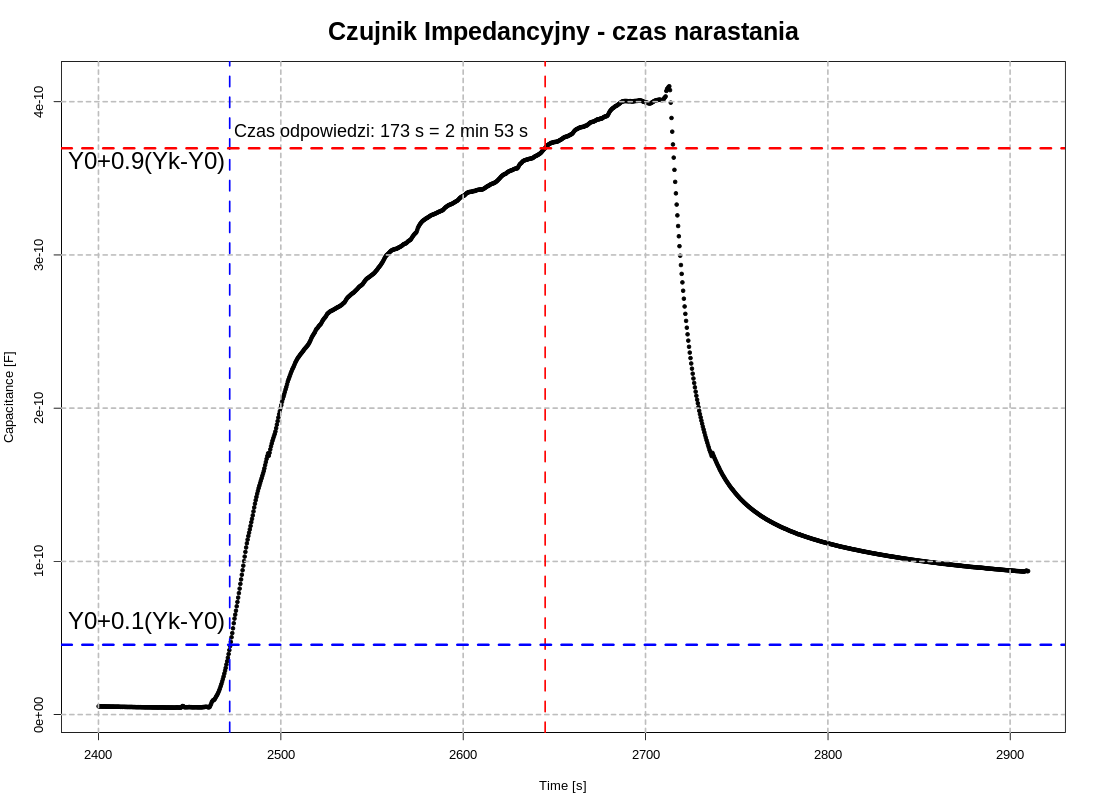
\includegraphics[scale = 0.35]{/home/bork/IdeaProjects/LatexProjects/src/PodstawyTechnikiSensorowej/Lab5/Img/rising.png}}
    \noindent\makebox[\textwidth]{
        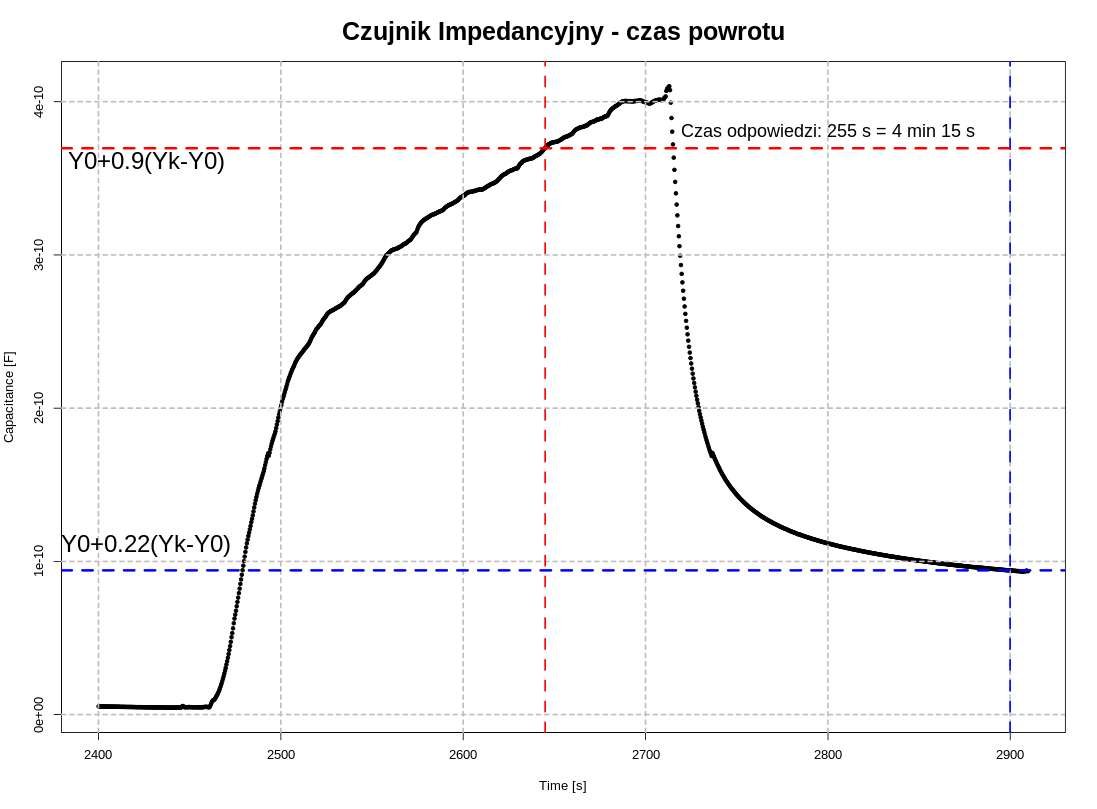
\includegraphics[scale = 0.35]{/home/bork/IdeaProjects/LatexProjects/src/PodstawyTechnikiSensorowej/Lab5/Img/fall.png}}
    \indent Oba te czasy to czas który potrzebuje czujnik aby przejść z 10\% różnicy wartości makymalnej i minimalnej pomiaru do 90\%
    tej wartości. W przypadku czasu odpowiedzi jest to zbocze narastające a dla czasu powrotu jest to zbocze opadajace. Gdyż nie sygnałowi
    opadającemu nie udało się spaść do poziomu 10\% różnicy maksimum i minimum, wykorzystano najniższą wartość jaką osiągną czujnik przed włożeniem
    go do kolejnej atmosfery. Wartość ta to 22\% różnicy maksimum i minimum.\\
    \subsection{Tabela z danymi}
    \begin{center}
        \Large\csvreader[tabular = |c|c|c|c|c|c|,
            table head = \hline  \textbf{Środowisko}  & \textbf{$RH_t$}& \textbf{$RH_m$}  & \textbf{$RH_k$} & \textbf{x [ppm]} & \textbf{\boldmath$p_w$ [Pa]}  \\\hline,
            late after line = \\\hline
        ]{Dane/output.csv}{}{
            \csvcolii & \csvcoliii & \csvcoliv & \csvcolviii  & \csvcolv & \csvcolix
        }
    \end{center}
    \noindent Gdzie:
        {\footnotesize
    \begin{itemize}
        \setlength\itemsep{0em}
        \item[] \textbf{$RH_t$} - teoretyczna wartość wilgotności powietrza w kolbie,
        \item[] \textbf{$RH_m$} - zmierzona wartość wilgotności powietrza w kolbie,
        \item[] \textbf{$RH_k$} - skorygowana wartośc wilgotności powietrza dla temperatury 25 [$C^\circ$]
        \item[] \textbf{$x$} - zawartość pary wodnej w powietrzu
        \item[] \textbf{$p_w$} - ciśnienie cząsteczkowe pary wodnej
    \end{itemize}}
\newpage
    \section{Wnioski}
    \par Na podstawie przeprowadzonych doświadczeń można wysunąć następujące wnioski:
    \begin{itemize}
        \item Czujniki wilgotności charakteryzują się różnymi charakterystykami wartości zmieniającej się wraz ze zmianą wilgotności. Dla czujnika
        pojemnościowego zmiana ta była liniowa podczas gdy dla czujnika impedacyjnego była to zmiana nieliniowa.
        \item Można zauważyć różnice między ciśnieniem cząsteczkowym pary wodnej a zawartością pary wodnej w powietrzu. Obie wartości są ze sobą
        skorelowane ponieważ obie opisują obecność molekół wody w mieszaninie gazów. Nie rosną one jednak równomiernie. Ciśnienie cząsteczko opisuje
        ciśnienie jakie wywiar para wodna w mieszaninie gazów podczas gdy zawartość pary wodnej opisuje procentową ilość pary w gazie.
        \item Czas odpowiedzi i powrotu dla tych czujników jest dość długi bo wynosił w naszym przypadku aż kilka minut. Czujniki te więc nie nadają sie
        do pomiarów w systemach które wymagają natychmiastowej odpowiedzi np.: systemy medyczne, systemy bezpieczeństwa.
    \end{itemize}




    %Bibliografia
    \vfill
    \footnotesize
    \begin{thebibliography}{3}
        \bibitem{texbook1}
        https://en.wikipedia.org/wiki/Partial\_pressure
        \bibitem{texbook2}
        https://www.engineeringtoolbox.com/relative-humidity-air-d\_687.html
        \bibitem{texbook3}
        https://en.wikipedia.org/wiki/Water\_vapor
    \end{thebibliography}
\end{document}